\documentclass[12pt,a4paper]{article}
\usepackage[utf8]{inputenc}
\usepackage[T1]{fontenc}
\usepackage[francais]{babel}
\usepackage{amsmath}
\usepackage{amsfonts}
\usepackage{amssymb}
\usepackage{xcolor}
\usepackage{graphicx}
\usepackage[top=2.00cm]{geometry}
\usepackage{titlesec}
\usepackage{fancyhdr}
\usepackage{multicol}
\usepackage{titling}
\graphicspath{{C:/Users/Sylvain/AppData/Roaming/texstudio/templates/user/}{./res/}}

%%modif des titres de section diminuer la taille
\renewcommand{\thesection}{\Roman{section}}
\titleformat{\section}
{\normalfont\bfseries\Large\scshape}{\thesection}{1em}{}
\titleformat{\subsection}
{\normalfont\bfseries\large}{\thesubsection}{1em}{}

\addto{\captionsfrench}{\renewcommand{\abstractname}{}}


%todo CONFIG
\author{Sylvain Finot}
\title{Initiation à la recherche :\\[5pt] \scshape "The Rattleback revisited"}
\date{\today}
\fancypagestyle{firststyle}{
	\fancyhf{}
	\setlength{\footskip}{2cm}
	\renewcommand{\headrulewidth}{0pt}
	\cfoot{\textcolor{lightgray}{\theauthor \ | Initiation à la recherche | Mars 2017}}
	\rfoot{\thepage}
}
\pagestyle{firststyle}

\makeatletter
\def\@maketitle{
	\begin{center}
		
		% NoLogo
		% \vspace*{+2cm}
		
		% Corner Logo
		% \begin{flushright}
		%  
\includegraphics[width=40mm]{logo_corner}\\[4ex]
		% \end{flushright}
		
		% Top Logo
		
\includegraphics[scale=0.3]{logo_top}
		
		
		{\LARGE \@title }\\[4ex]
		{\large \@author}\\[4ex]
		{\large \@date}\\[8ex]
		\rule{\linewidth}{0.4pt}
	\end{center}
}


%matrices configurables \begin{pmatrix}[2pt]
\renewcommand*\env@matrix[1][\arraystretch]{%
	\edef\arraystretch{#1}%
	\hskip -\arraycolsep
	\let\@ifnextchar\new@ifnextchar
	\array{*\c@MaxMatrixCols c}}
\makeatother


\begin{document}
	%todo mettre Intro sur nouvelle page?
	\maketitle
	\thispagestyle{firststyle}
	\begin{abstract}
		Cet article est essentiellement basé sur le travail de William Case et Sahar Jalal concernant le mouvement particulier du rattleback.
	\end{abstract}
	\section{Introduction}
	Un rattleback, aussi appelé anagyre ou "Celtic stone", est un objet généralement en forme de canoë, qui a la particularité d'avoir un sens de rotation stable et un sens instable autour de l'axe vertical.
	\begin{figure*}[h]
		\centering
		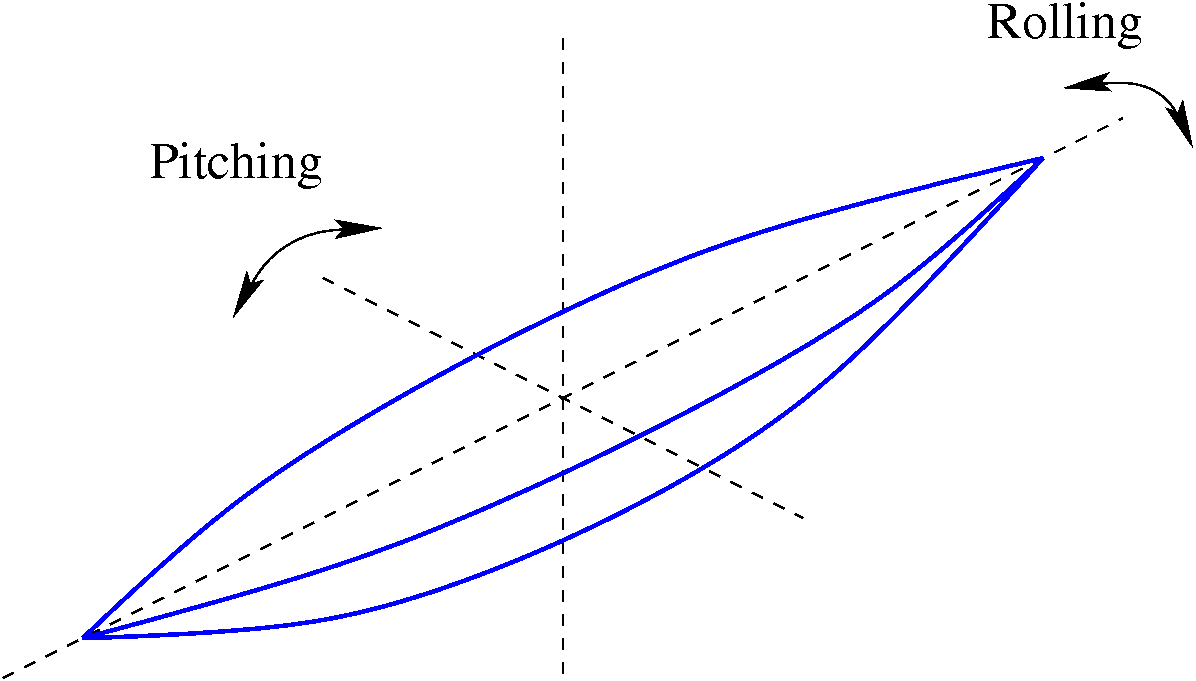
\includegraphics[scale=0.2]{Rolling-pitching}
		\caption[]{Représentation simpliste d'un rattleback}
		\label{fig:rolling-pitching}
	\end{figure*}
	
	Autrement dit, si on le met en rotation dans le "bon" sens, le mouvement continue jusqu'à immobilisation due aux forces de frottement. En revanche, si on le met en rotation dans le "mauvais" sens, très vite, l'objet oscille violemment ("rattle"), s'arrête, puis repart en sens inverse (i.e, le "bon" sens). Autre particularité, si on fait osciller le rattleback selon son petit axe (l'axe "pitching" ci-dessus), il entre en rotation dans le bon sens de rotation.
	
	Cet objet, par son mouvement paradoxal, est parfois retrouvé comme accessoire de magicien.
	Il a également fasciné grand nombre de physiciens et de mathématiciens. Les premières publications a ce sujet datent de 1896 par Gilbert Walker et bon nombre de publications actuelles (XXI$^{e}$ siècle) se basent sur les travaux de Sir Hermann Bondi, "The Rigid Body Dynamics of Unidirectional Spin" de 1986.
	\subsection{Un problème de symétrie.}
	Bien que le mouvement du rattleback soit surprenant et fascinant, il n'y a rien de magique dans cet objet. Ses propriétés sont dues à un problème de symétrie. En effet, le rattleback est un objet asymétrique.
	
	Il existe deux manières de concevoir un rattleback : on peut décider de prendre une répartition de masse homogène, et dans ce cas, on brise la symétrie en modifiant le volume. On peut aussi choisir de conserver les symétries du volume et de "cacher" l'asymétrie en appliquant une répartition inhomogène de la masse avec par exemple des cavités. L'étude faite ici concerne le cas de répartition de masse homogène.
	
	Le problème étant complexe, il faut faire un certain nombre d'hypothèses pour pouvoir espérer le résoudre.
	%todo : HYPOTHESES
	On considère que le point de contact entre le rattleback et le support est au repos.
	%Conservation de l'E (28 29)
	
	Pour simplifier le traitement du problème, on peut le découper en deux parties.\\
	La première consiste à étudier comment, à partir de rotation, le rattleback se met en oscillation. %D'une certaine manière, on peut voir cela comme une conversion d'énergie.\\
	La deuxième partie, on s'intéresse au cas contraire, comment à partir d'oscillations le rattleback passe-t-il en rotation.
	\section{Oscillations}
	Dans cette première partie de l'étude, on considère que le rattleback est initialement en rotation selon l'axe vertical sans aucune oscillation. On cherche alors a expliquer pourquoi et comment ce mouvement se transforme en oscillation.
	%L'idée est de mettre en équation le changement 
	En ce qui concerne l'aspect calculs, l'étude se fait dans le référentiel du centre de masse. Ce référentiel étant en rotation, il faut en tenir compte pour certains calculs.\\
	Le repère utilisé a pour origine le centre de masse et comme axes, les axes de symétrie (en terme de distribution de masse).\\
	\begin{figure}[h]
		\centering
		\caption{Le rattleback vu de dessus. La répartition de masse ne respecte pas la symétrie de la forme.}{Crédit : Case \& Jalal}
		\label{fig:mass-repartition}
		\includegraphics[width=0.7\linewidth]{"mass repartition"}
	\end{figure}
	
	L'étude commence en s'intéressant au point de contact en le rattleback et le support. On note indique cette position par le vecteur $\vec{r}=(x,y,z)$. Après calculs, et en supposant que $x$ et $y$ ne sont pas trop éloignés de l'origine, on peut trouver une expression de la composante z.
	
	\begin{equation}
	z=a\left[ 1-\dfrac {1} {2}p\left( \dfrac {x} {a}\right) ^{2}-q\dfrac {xy} {a^{2}}-\dfrac {1} {2}s\left( \dfrac {y} {a}\right) ^{2}\right]
	\label{eq:z}
	\end{equation}
	
	On définit également le vecteur $\vec{u}$ qui est le vecteur unitaire normal à la surface qui est donc constant dans le référentiel du laboratoire. Concrètement, il s'agit "simplement" du vecteur unitaire définissant l'axe vertical dans le référentiel du laboratoire.\\
	
	En exprimant ce vecteur dans le référentiel du centre de masse, on obtient l'expression suivante :
	%todo d'ou vient l'idée de différentielle ?
	\begin{equation}
	\vec{u}=-\left(\dfrac{px+qy}{a},\dfrac{qx+sy}{a},1\right)
	\label{eq:uNormal}
	\end{equation}
	Où : \\
	\begin{tabular}{ll}
		$p$ &la courbure selon $x$\\
		$s$ &la courbure selon $y$\\
		$a$ &la distance entre le centre de masse et le point le plus bas du rattleback au repos\\
		$q$ &le facteur représentant l'asymétrie de l'objet
	\end{tabular}
	\\
	
	L'expression est un peu compliquée, en effet le rattleback étant plus ou moins un demi-ellipsoïde, il semble normal de retrouver les paramètres dans l'expression de $\vec{u}$.\\
	
	Par la suite, en utilisant la formule de Bour \eqref{eq:bour}, et disant que $\vec{u}$ est constant dans le référentiel du laboratoire \eqref{eq:uConstant}, on peut trouvé une expression de $\vec{\omega}$(Calculs détaillés dans la partie \ref{subsec:omega})\\
	\begin{multicols}{2}
		\setlength\columnseprule{0.5pt}
		\noindent
		\begin{flalign}
		\dfrac{d\vec{A}}{dt}&=\dot{\vec{A}}+\vec{\omega}\times\vec{A}&
		\label{eq:bour}\\[1em]
		\dfrac{d\vec{u}}{dt}&=0&
		\label{eq:uConstant}
		\end{flalign}
		\vfill\null
		\columnbreak
		\noindent
		\begin{equation}
		\vec{\omega}=\dfrac{1}{a}\begin{pmatrix}[2]
		q\dot{x}+s\dot{y}-n(px+qy)\\
		-p\dot{x}+q\dot{y}-n(qx+sy)\\
		- na
		\end{pmatrix}
		\end{equation}
	\end{multicols}
	
	
	On peut alors trouver une expression de la vitesse, en effet : $\vec{v}=-\vec{r}\times\vec{\omega}$.\\
	\textbf{Remarques} :
	\begin{enumerate}
		\item Pour garder uniquement les termes du 1er ordre, cela revient à prendre $\vec{r}=(x,y,a)$ puisqu’ $z=a$ au premier ordre.
		
		\item Si l'on veut être plus précis, la formule de Bour~\eqref{eq:bour} s'écrit de la manière suivante:  
		$$\left( \frac{d\vec{A}}{dt} \right)_{(R)}=\left ( \frac{d\vec{A}}{dt}  \right)_{(R')}+\vec{\Omega}_{(R'/R)}\wedge\vec{A}$$
		Ou R est le référentiel dit "fixe" (galiléen) et R' le référentiel mobile
	\end{enumerate}
	
	À partir de ce stade, la procédure devient plus "classique".\\
	En appliquant la deuxième loi de Newton:
	\begin{align*}
	\Sigma\vec{F}  &= m\vec{a}\\
	\iff\vec{F_c}+\vec{P} &= m\dfrac{d\vec{v}}{dt}
	\intertext{Ou encore:}
	\iff\vec{F_c}-mg\vec{u}=\dfrac{d\vec{p}}{dt}
	\end{align*}
	% l'accélération du barycentre dans le référentiel du laboratoire à l'aide de \eqref{eq:bour}.
	En prenant le produit vectoriel de l'expression ci-dessus avec $\vec{r}$ on obtient:
	\begin{equation}
	\dfrac{d\vec{L}}{dt}=m(\vec{r}\times\dfrac{d\vec{v}}{dt}+g\vec{r}\times\vec{u})
	\end{equation}
	Mais en utilisant la formule de Bour \eqref{eq:bour}, on peut également obtenir:
	$$\dfrac{d\vec{L}}{dt}=\dot{\vec{L}}+\vec{\omega}\times\vec{L}$$
	Remarque : Pour obtenir quelque chose d'intéressant, il semblerait qu'il faille conserver les termes d'ordre 2 dans cette expression.\\
	
	Ainsi, on obtient
	\begin{equation}
	m(\vec{r}\times\dfrac{d\vec{v}}{dt}+g\vec{r}\times\vec{u})=\dot{\vec{L}}+\vec{\omega}\times\vec{L}
	\end{equation}
	En calculant le terme explicitement le terme de droite, on obtient deux équations différentielles couplées.
	
	Dans un premier temps, les auteurs de l'article considèrent que le rattleback est au repos et qu'il ne possède pas d'asymétrie. (i.e $q=n=0$). On peut alors résoudre ces équations plus simplement et trouver les pulsations propres de l'objet. \\
	
	Par la suite, on reprend les équations différentielles en considérant l'asymétrie et la rotation. Le point le plus important pour les auteurs n'est pas la précision sur les pulsations mais de mettre en évidence les termes qui déstabilisent les oscillations.  
	
	
	\section{Rotation engendrée par des oscillations}
	Expliquer la rotation engendrée par des oscillations est plus simple que considérer l'inversement du sens de rotation.\\
	Pour expliquer ce phénomène, il faut considérer un mouvement d'oscillation autour de l'axe x, et aucune rotation autour de l'axe z.
	\begin{figure}
		\centering
		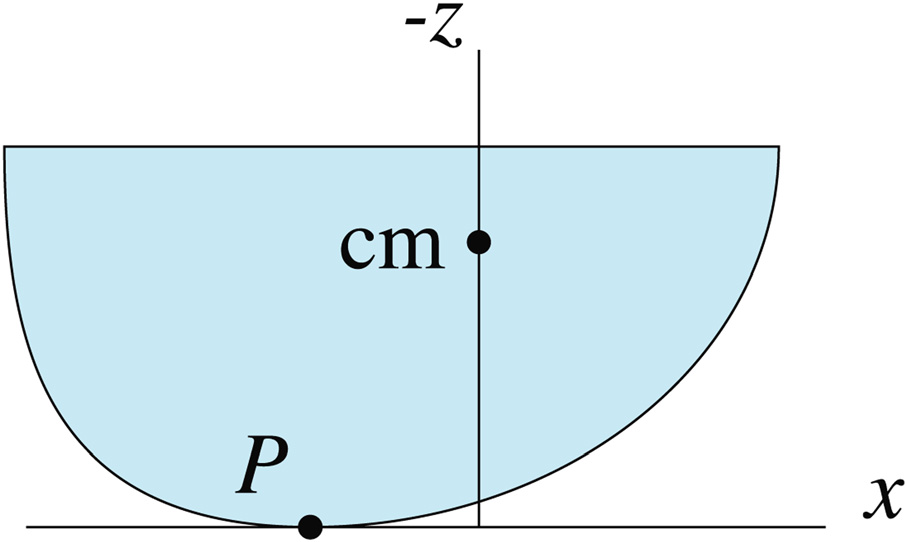
\includegraphics[width=0.7\linewidth]{res/coupe}
		\caption{Vu en coupe du rattleback pendant une osccillation autour de l'axe x}{Crédit : Case \& Jalal}
		\label{fig:coupe}
	\end{figure}
	Le centre de masse n'ayant pas la même abscisse selon les $x$, le poids de celui-ci crée un couple au point de contact. Voir figure~\ref{fig:coupe}. Ce couple tend à mettre en rotation le rattleback selon l'axe y.\\
	L'expression de ce couple au point P est donnée par :
	\begin{equation}
		\dfrac{dL_{py}}{dt}=-mgx=\dfrac{mgqy}{p}
	\end{equation}
	Dans le référentiel du centre de masse, au point P et au premier ordre, on a :
	\begin{align}
%		\vec{v}	&=\vec{r}\times\vec{\omega} \nonumber \\
%				&\approx\left[0,0,a\right]\times\\
		v_x&=a \omega_y\\
		\intertext{D'où}
		\dfrac{dv_x}{dt}&=a\dfrac{d\omega_y}{dt}
	\end{align}
	%Dans ref du rattleback le point de contact $v_x=a\omega_y$ d'ou eq (31) (d/dt)
	%
	%acceleration => force => couple si "bras de levier"
	%le couple mets en rotation
	\section{Explications et vérifications des calculs}
	\label{sec:calculs}
	Dans cette section, on essaie de retrouver une partie des expressions données par les auteurs, en détaillant au possible les méthodes et les hypothèses pour y parvenir.\\
	Par alléger l'écriture, on pose la définition suivante :
	$$\dfrac{\partial}{\partial x}\equiv\partial_x$$ 
	\subsection{Vecteur normal}
	La formule \eqref{eq:z} est liée à la forme d'ellipsoïde. Je n'ai pas compris pourquoi, mais on trouve le vecteur normal $\vec{u}$ \eqref{eq:uNormal} en prenant le gradient de \eqref{eq:z}. En effet :
	\begin{align*}
	\vec{\nabla}\cdot z &= \begin{pmatrix}
	\partial_x\\
	\partial_y\\
	\partial_z
	\end{pmatrix}
	\cdot
	a\left( 1-\dfrac {1} {2}p\left( \dfrac {x} {a}\right) ^{2}-q\dfrac {xy} {a^{2}}-\dfrac {1} {2}s\left( \dfrac {y} {a}\right) ^{2}\right)\\
	&=-\left(\dfrac{px+qy}{a},\dfrac{qx+sy}{a},1\right)
	\end{align*}
	\textbf{Remarque : } Il est dit dans l'article que $\vec{u}$ est le vecteur normal unitaire.
	\begin{quotation}
		<<upward-pointing unit normal u at that point is given, to first
		order in x and y, by...>>
	\end{quotation}
	Or, simplement en constatant que $u_z=1$, on en déduit que le vecteur n'est pas normé. Il faudrait prendre:
	\begin{align*}
	\vec{v} &=\dfrac{\vec{u}}{||u||}\\
	&=\dfrac{\vec{u}}{\sqrt{\left(\dfrac{px+qy}{a}\right)^2+\left( \dfrac{qx+sy}{a}\right)^2+1}}
	\end{align*}
	Cette petite "erreur" n'a pas d'importance sur la suite des calculs puisque la suite découle des équations suivantes :
	%todo : Faire ca sur 2 cols ?
	\begin{align*}
	\dfrac{d\vec{A}}{dt}&=\dot{\vec{A}}+\vec{\omega}\times\vec{A}\\[4pt]
	\dfrac{d\vec{v}}{dt}&=0
	\intertext{il vient alors :}
	\dfrac{d\vec{v}}{dt}&=\dot{\vec{v}}+\vec{\omega}\times\vec{v}\\
	&=\alpha\dot{\vec{u}}+\vec{\omega}\times\alpha\vec{u}\\
	&=\alpha(\dot{\vec{u}}+\vec{\omega}\times\vec{u})\\
	\intertext{D'où}
	\dot{\vec{u}}+\vec{\omega}\times\vec{u}=0 &\iff \dot{\vec{v}}+\vec{\omega}\times\vec{v}=0
	\end{align*}
	
	\subsection{Vecteur rotation $\vec{\omega}$}
	\label{subsec:omega}
	Pour trouver une expression de $\vec{\omega}$ nous avons besoin d'une propriété sur le produit vectoriel.
	\begin{equation}
	\vec{a}\times(\vec{b}\times\vec{c})=\vec{b}(\vec{a}\cdot\vec{c})-\vec{c}(\vec{a}\cdot\vec{b})
	\end{equation}
	Selon les équations \eqref{eq:bour} et \eqref{eq:uConstant} on a:
	\begin{align*}
	\dot{\vec{u}}+\vec{\omega}\times\vec{u}         &= 0\\
	\vec{u}\times(\dot{\vec{u}}+\vec{\omega}\times\vec{u})     &= 0\\
	\vec{u}\times\dot{\vec{u}}+\vec{u}\times(\vec{\omega}\times\vec{u})  &= 0\\
	\vec{u}\times(\vec{\omega}\times\vec{u})        &=-\vec{u}\times\dot{\vec{u}}\\
	\vec{\omega}(\vec{u}\cdot\vec{u})-\vec{u}(\vec{u}\cdot\vec{\omega})  &=\dot{\vec{u}}\times\vec{u}\\
	\intertext{En prenant $||\vec{u}||=1$ et en posant $\vec{u}\cdot\vec{\omega}\equiv n$}
	\vec{\omega}=\dot{\vec{u}}\times\vec{u}+n\vec{u}
	\end{align*}
	
	L'idée de poser $\vec{u}\cdot\vec{\omega}\equiv n$ m'a posé pas mal de problèmes de compréhension. Je me demandais quel en était l'intérêt, jusqu'à ce que je calcule explicitement $\vec{\omega}$.\\
	\bgroup
	\addtolength{\jot}{5pt}
	\begin{align*}
	\vec{\omega} &= \dot{\vec{u}}\times\vec{u}+n\vec{u}\\
	&=\begin{pmatrix}[2]\dfrac{p\dot{x}+q\dot{y}}{a}\\\dfrac{q\dot{x}+s\dot{y}}{a}\\0\end{pmatrix} \times \begin{pmatrix}[2]\dfrac{px+qy}{a}\\\dfrac{qx+sy}{a}\\1\end{pmatrix} -n\begin{pmatrix}[2]\dfrac{px+qy}{a}\\\dfrac{qx+sy}{a}\\1\end{pmatrix}\\
	%
	&=\begin{pmatrix}[2]
	\dfrac{q\dot{x}+s\dot{y}}{a}-n\dfrac{px+qy}{a}\\
	-\dfrac{p\dot{x}+q\dot{y}}{a}-n\dfrac{qx+sy}{a}\\
	\left(\dfrac{p\dot{x}+q\dot{y}}{a}\right)  \left(\dfrac{qx+sy}{a}\right)  - \left(\dfrac{q\dot{x}+s\dot{y}}{a}\right)  \left( \dfrac{px+qy}{a}\right)  - n
	\end{pmatrix}
	\end{align*}
	Il semblerait que les auteurs aient fait une hypothèse simplificatrice, les termes sous forme de fraction sont d'ordre 1. On a donc $\omega_z\approx-n$ (le produit est d'ordre 2). D'où
	\begin{equation}
	\vec{\omega}=\dfrac{1}{a}\begin{pmatrix}[2]
	q\dot{x}+s\dot{y}-n(px+qy)\\
	-p\dot{x}-q\dot{y}-n(qx+sy)\\
	- na
	\end{pmatrix}
	\end{equation}
	\egroup
	Vérifions si on peut considérer les hypothèses comme valides :
	
	
	On rappelle que $x$ et $y$ représentent les coordonnées horizontales et verticales du point de contact par rapport au centre de masse. On se convint assez facilement que cet écart au centre de masse et petit par rapport aux dimensions de l'objet.On prendra en ordre de grandeur le millimètre.
	
	
	Nous n'avons pas d'information particulière sur les $\dot{x}$ et $\dot{y}$. Cependant les auteurs souhaitent résoudre le problème pour de petites vitesses.
	
	\begin{multicols}{2}
		\noindent
		\begin{align*}
		x&\approx y \approx 10^{-3}m&\\
		p&=0,923&\\
		s&=0,034&\\
		q&=0,1&\\
		a&=7,1.10^{-3}m&\\
		\end{align*}
		\columnbreak
		\begin{align*}
		\dfrac{qx+sy}{a}&\approx0,06\\[2em]
		\dfrac{px+qy}{a}&\approx0,27
		\end{align*}
	\end{multicols}
	\vspace*{-3em}
	On peut supposer que les termes en $\dot{x}$ et $\dot{y}$ sont également du même ordre.\\
	L'hypothèse de considérer $\omega_z\approx-n$ semble plutôt bonne.
	
	%todo calc de v ?
	
	
	\subsection{Moment cinétique et moments de force}
	\label{subsec:moments}
	On cherche à obtenir une relation entre moments de forces (exprimés au barycentre) et moment cinétique. Les quantités sont exprimées dans le référentiel du laboratoire supposé galiléen.
	On part de:
	\begin{align*}
	\vec{L}     &= \vec{r}\times \vec{p}\\
	\iff\dfrac{d\vec{L}}{dt} &= \dfrac{d}{dt}(\vec{r}\times \vec{p})\\
	\iff\dfrac{d\vec{L}}{dt} &= \dot{\vec{r}}\times \vec{p}+\vec{r}\times \dfrac{d\vec{p}}{dt}\\
	\intertext{Or $\vec{p}$ et $\dot{\vec{r}}$ sont colinéaires $\implies \dot{\vec{r}}\times \vec{p} = 0$}
	\iff\dfrac{d\vec{L}}{dt} &= \vec{r}\times \dfrac{d\vec{p}}{dt}
	\end{align*}
	De plus $\dfrac{d\vec{p}}{dt}=\Sigma\vec{F}$ (2$^{\mathrm{eme}}$ loi de Newton)
	\begin{equation}
	\iff\dfrac{d\vec{L}}{dt} = \vec{r}\times\Sigma\vec{F}
	\end{equation}
	On retrouve en fait le théorème du moment cinétique.
\end{document}
% Ils disent qu'ils n'ont pas forcément été plus loin dans l'analyse que leur prédeccesseur mais qu'a l'aide de bonnes approximations, ils ont pu grandement alleger les calculs et ainsi arrivé plus rapidement et facilement a un resultat

%todo : ouverture sur autres objets étranges. Gömböc
